
% Take extra care in avoiding ``expansion'' -- stick to ``evaluation''

\todo{Tie-breaking or tie-breaking? Tie-Breaking.}
\todo{Inadmissible or non-admissible? Inadmissible.}
\todo{last frontier or final frontier?}

\begin{abstract}
% this current version is intentionally ambiguous as possible
Despite the recent improvements in admissible heuristic search techniques
in classical planning, the exponential growth of
the size of search plateaus in A* is unavoidable.
We investigate tie-breaking strategies for A*, and propose simple yet effective methods for improving performance on domains with large search plateaus.

%%  % 
%% We investigate various existing myth on tie-breaking
%% strategies and propose simple yet effective methods for improving the
%% search performance within plateau.
%%  % 
%%  % 
%%  They do not depend on any particular heuristic, nor
%%  on multi-heuristic portfolio.
%%  They work even if the heuristic
%%  function no longer provides useful information.
%%  % Moreover, they do not even try to obtain any further information from
%%  % the domain.
%%  We empirically evaluate our strategies against state-of-the-art admissible planner.
\end{abstract}

\section{Introduction}
%Motivation: The Importance of the Last Frontier in A* and Domains with Large Plateaus
\label{sec-1}

%\subsubparagraph{\astar and perfect heuristics}

This paper investigates tie-breaking strategies for \astar.
\astar is a standard search algorithm for finding an optimal-cost path 
from an initial state $s$ to some goal state $g \in G$ in a search space represented as a graph \cite{hart1968formal}.
In each iteration, \astar selects and \emph{expands} a node $n$ from the OPEN priority queue.
$n$ is the node which has the lowest $f$-cost in OPEN, where for node $n$, $f(n)$ is the sum of  $g(n)$, the cost of the current path from the start state to $n$, and $h(n)$, a heuristic estimate of the cost from $n$ to a goal state.
\astar returns an optimal solution when $h$ is admissible, i.e., when $h \leq h^*$, where $h^*$ is the true distance to the goal.


In order to guarantee solution optimality, \astar expands all
nodes with $f(n) < f^*$, where $f^*$ is the cost of the optimal solution.
%All nodes with $f(n) = k$ are expanded before any node with $f(n) > k$ are expanded.
%Thus, after all nodes with $f(n) < f^*$ have been expanded, 
\astar expands \emph{some} of the nodes with $f(n) = f^*$, and never expands a node with $f(n) > f^*$.
Thus, the \emph{effective search space of \astar} is the set of nodes with 
$f(n) \leq f^*$, and
much of the work in the AI search and planning literature  has focused
on reducing the size of this effective search space by
developing more accurate, admissible heuristic functions.

In many problems, the size of the \emph{last frontier}, the set of nodes with $f(n)=f^*$, accounts for a significant portion of $A$.
\refig{fig:plateau-noh} plots the number of states with $f(n) = f^*$ (y-axis)
versus the number of states with $f(n) \leq f^*$
for a set of 1104 benchmark problem instances from the ICAPS International Planning Competition (IPC1998-2011).
For many instances in \refig{fig:plateau-noh},  a large fraction of the nodes with $f(n) \leq f^*$ have $f(n)=f^*$.
For example, in the Openstacks domain, almost all states with $f(n) \leq f^*$ have cost $f^*$.
In such domains, the behavior of \astar on the last frontier is critical -- the policy for deciding which nodes to expand in the last frontier can have a significant impact on the performance of \astar.

\begin{figure}[tb]
 \centering \relsize{-3} 
 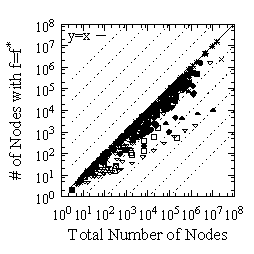
\includegraphics{tables/aaai16-frontier/aaai16prelim3/lmcut_frontier_noh-front-mono.pdf}
 \caption{
 The number of the nodes with cost $f=f^*$ (y-axis) compared to the
 total number of nodes in the search space with cost $f\leq f^*$ on 1104 IPC benchmark problems
(search space analyzed using Fast Downward with \lmcut heuristic, slightly modified to generate all nodes with cost $f^*$).}
\label{fig:plateau-noh}
\end{figure}

In this paper, we focus on the \emph{tie-breaking} policy used by
\astar, which selects a node to expand among nodes with the same
$f$-cost.  Since \astar expands all nodes with $f$-cost less than $f^*$
before expanding any nodes with cost $f^*$, the tie-breaking policy only
affects performance when considering the last frontier (nodes with cost
$f^*$).  Although there has not been much previous \emph{in-depth} work
on tie-breaking policies for admissible search algorithms, it is widely believed that among nodes with
cost $f(n) = f^*$, ties should be broken according to $h(n)$, i.e.,
nodes with smaller $h$ values should be expanded first.  While this is a
useful rule of thumb in many domains, it turns out that tie-breaking
requires more careful consideration, particularly for problems with
large \emph{plateaus} -- regions of the search space with the same $f$-cost.
\emph{Note that all tie-breaking strategies investigated in this paper
maintain the admissibility of the search because it only affects the node expansion
order among the nodes with the same $f$-cost.}

We first empirically evaluate widely used tie-breaking strategy for \astar, and show that 
% 
(1) a Last-In-First-Out (\lifo) policy for breaking ties among nodes with the same $f$ {\bf and h?} value tends to be more efficient than an a First-In-First-Out (\fifo) policy, and 
% 
(2) with \lifo implementation, tie-breaking according to $h$, which
frequently appears in the heuristic search literature, has little 
impact on the performance.
% 
%% Remove?
% \todo[
% Third, the \lifo-based bucket implementation and $h$-based tie-breaking
% both share the greedy search pattern within the plateau of the
% search space.]{this is not shown yet. how to show it? xy-plot of the node
% evaluation order?}

These experiments show that there are significant performances differences among tie-breaking strategies
when domains have zero-cost actions.  While there are relatively few domains with zero-cost actions in the existing IPC benchmark sets, we argue that this is a historical accident, and that in fact, many unit-cost domains may be more appropriately modelled using zero-cost actions.
%Through these experiments, we points out a bias in the current set of
%benchmark domains and the importance of tie-breaking in
%the more practical cost-minimization problems.

Next, in order to solve those cost-minimization problems with zero-cost actions,
we propose 
tie-breaking methods
based on a notion of \emph{depth} within the plateau, which corresponds to the number of steps 
a node is from the ``entrance'' to the plateau region.
We show that one strategies called RandomDepth provides a significant performance improvement
compared to the other tie-breaking strategies using the same heuristic function.

Finally, we show the robustness of our tie-breaking strategies
against a particular action ordering in the domain definition.
Our depth-based tie-breaking is a part of multi-level tie-breaking strategy,
and we show that the notion of depth is the principal factor in determining performance.

% XXX It's doubtful that anybody would believe that machine-level efficiency of LIFO (compared to FIFO) is important in domain-independent planning.
%At the same time, we show that 
%the performance of above \lifo tie-breaking can be explained by its
%depth-first strategy, and the other characteristics of \lifo such as
%machine-level efficiency have little effect on the performance.

%% Above describes the enough detail of the paper structure?

\section{Tie-breaking Strategies in \astar}

%Aside from the heuristic function, most best-first family of search
%algorithms, including \astar, IDA* and so on, have a tie-breaking criteria which is used
%when two nodes have the same $f$ value.

If multiple nodes with the same $f$-cost are possible, \astar
must implement some tie-breaking policy (either
explicitly or implicitly) which selects from among these nodes.
The early literature on heuristic search seems to have been mostly agnostic on the issue of tie-breaking.
The original paper proposing \astar, as well as Nilsson's
subsequent textbook states: ``Select the open node $n$ whose value $f$
is smallest. Resolve ties arbitrarily, but always in favor of any [goal
node]'' \cite[p.102 Step 2]{hart1968formal} \cite[p.69]{Nilsson71}.
% Although it is possible to interpret this to imply $h$-based tie-breaking
% since goal nodes are the special case where $h=0$,
% they make no further metion of tie-breaking.
Pearl's textbook on heuristic search specifies that best-first search should ``break ties arbitrarily'' (\citeyear{pearl1984heuristics}, p.48, Step 3), but does not specifically mention tie-breaking for \astar.
Interestingly, in his analysis of IDA*, Korf mentions that ``If \astar employs the tie-breaking rule of 'most-recently generated', it must also expand the same nodes [as IDA*]'' (\citeyear{korf1985depth}) -- this purely \lifo ordering is the first explicit mention we found of a tie-breaking policy not based on $h$.

In recent years, tie-breaking accoording to $h$-values has become ``folklore'' in the search community.
\citeauthor{hansen2007anytime} state that ``It is well-known 
that \astar achieves best performance when it breaks ties
in favor of nodes with least h-cost'' \cite{hansen2007anytime}.
\citeauthor{holte2010common} writes ``\astar breaks ties in favour
of larger g values, as is most often done'' \cite[note that since $f=g+h$,
preferring large $g$ is equivalent to preferring smaller $h$](\citeyear{holte2010common}.
% \citeauthor{felner2011inconsistent} also assume ``ties are broken in
% favor of low h-values'' in describing Bidirectional Pathmax for \astar.
In their detailed survey/tutorial on efficient \astar implementations,
\citeauthor{burns2012implementing} (\citeyear{burns2012implementing})
also break ties ``preferring high $g$.''
%% this could be moved to later analysis
% They further write: ``The reasoning is that the goal can be found more
% quickly in the final $f$ layer of search''.
Thus, tie-breaking according to $h$-values appears
to be ubiquitous in practice.

Although the standard practice of tie-breaking according to $h$ might be
sufficient in some domains, further levels of tie-breaking (explicit or
implicit) are required if multiple nodes can have the same $f$ and
$h$ values.
%% we do, in Roger, Helmert
% We are not aware of any work that explicitly mentions 2nd-level tie-breaking.
While the survey of efficient \astar implementations in \citeauthor{burns2012implementing} did not explicitly mention 2nd-level tie-breaking, their code first breaks ties according to $h$, and then breaks remaining ties according to a \lifo policy (most recently generated nodes first).\footnote{https://github.com/eaburns/search}
Although not documented, their choice of a \lifo 2nd-level tie-breaking policy appears to be a natural consequence of the fact that the \lifo policy can be trivially, efficiently implemented in their two-level bucket (vector) implementation of OPEN.
In contrast, the current implementation of \sota \astar based planner Fast
Downward \cite{Helmert2006}\footnote{http://www.fast-downward.org}, and
the work by \cite{RogerH10} (based on Fast-Downward), uses
a \fifo second-level tie-breaking policy. 
Although we could not find an explanation, this is choice is mot likely due to their use of alternating OPEN lists, in which case the \fifo policy serves to provide a limited form of fairness.
%We could not find any explanation for this choice either.

%\citeauthor{Korf1985depth} uses $h$-based tie-breaking in the context of WA*
%\cite{korf1993linear}.  
% ** not sure how/where to put this..

\subsection{Reevaluating the Existing Strategies}


We tested various tie-breaking strategies throughout this paper.  In the
following sections, we use a convenient array-based notation of a
combination of tie-breaking strategy.  For example, $[f,h,\fifo]$ denotes
standard \astar with $h$-based first-level tie-breaking and \fifo
second-level tie-breaking.
%% I removed \fd because it is not yet proposed at this point

All planners are based on the latest Fast Downward code base, and all
experiments are run using 5 minutes runtime cutoff with 2GB memory
limit. Experiments were conducted on Xeon E5410@2.33GHz CPUs.
Our experimental results include 35 standard benchmark domains with 1104
problems.

We first compared two strategies $[f,h,\fifo]$, $[f,h,\lifo]$, which
first breaks ties according to $h$, and then applies \fifo or \lifo
second-level tie-breaking, respectively.
% The following will be necessary in a future version, if we use LOP:
%Although the search behavior of $[f,h,\fifo]$ corresponds to the default behavior of Fast Downward, this implementation differs 
%from the original, unmodified code because we enabled caching of $h$-values, so that reopened nodes refer to cached $h$-values.\footnote{The current Fast Downward code disables $h$-caching because its current implementation is not compatible with multiple admissible heuristics.}
%Thus, we also show results for unmodified Fast Downward -- as expected, $[f,h,\fifo]$ dominates unmodified FD.

The results for \astar using the LM-cut heuristic \cite{Helmert2009} are
shown in \reftbl{single-coverage} (Left).
Differences in coverage are observed in several domains.
Due to space limitation, we show only the domains
where there was any difference. Full data is available in the
supplemental material. \todo{probably better to show full results for this particular experiment}

\begin{table}[tb]
 \centering \relsize{-3}
 \begin{tabular}{|c|c|c|}
\hline      
 Domain & \rotatebox[origin=l]{90}{${\mbox{lmcut}}_{\mbox{ff}}$}   & \rotatebox[origin=l]{90}{${\mbox{lmcut}}_{\mbox{lf}}$}    \\
\hline      
 sum(1104) &  558 &  \textbf{565}  \\
\hline      
 {\relsize{-1}airport(50)} &  \textbf{27} &  26  \\
 {\relsize{-1}cybersec(19)} &  2 &  \textbf{3}  \\
 {\relsize{-1}mystery(30)} &  15 &  \textbf{16}  \\
 {\relsize{-1}openstacks-opt11(20)} &  11 &  \textbf{18}  \\
 {\relsize{-1}pipesworld-notankage(50)} &  \textbf{15} &  14 \\
\hline
\end{tabular}

 \begin{tabular}{|c|c|c|}
\hline      
 Domain & \rotatebox[origin=l]{90}{ff,noh}   & \rotatebox[origin=l]{90}{lf,noh}    \\
\hline      
 sum(1104) &  442 &  \textbf{556}  \\
\hline      
 {\relsize{-1}airport(50)} &  18 &  \textbf{26}  \\
 {\relsize{-1}cybersec(19)} &  0 &  \textbf{3}  \\
 {\relsize{-1}driverlog(20)} &  12 &  \textbf{13}  \\
 {\relsize{-1}elevators-opt11(20)} &  14 &  \textbf{15}  \\
 {\relsize{-1}freecell(80)} &  8 &  \textbf{9}  \\
 {\relsize{-1}logistics00(28)} &  16 &  \textbf{18}  \\
 {\relsize{-1}miconic(150)} &  68 &  \textbf{140}  \\
 {\relsize{-1}mprime(35)} &  19 &  \textbf{22}  \\
 {\relsize{-1}nomystery-opt11(20)} &  12 &  \textbf{13}  \\
 {\relsize{-1}openstacks-opt11(20)} &  11 &  \textbf{18}  \\
 {\relsize{-1}parcprinter-opt11(20)} &  12 &  \textbf{13}  \\
 {\relsize{-1}pathways(30)} &  4 &  \textbf{5}  \\
 {\relsize{-1}pipesworld-tankage(50)} &  7 &  \textbf{8}  \\
 {\relsize{-1}scanalyzer-opt11(20)} &  4 &  \textbf{10}  \\
 {\relsize{-1}visitall-opt11(20)} &  9 &  \textbf{10}  \\
 {\relsize{-1}woodworking-opt11(20)} &  6 &  \textbf{9}  \\
 {\relsize{-1}zenotravel(20)} &  9 &  \textbf{11} \\
\hline
\end{tabular}

 \caption{Experiments with 5 min, 2GB setting,
 comparing the coverages of \fifo and \lifo
 second-level tie-breaking, with (left) and without (right) the
 conventional first-level $h$ tie-breaking.  For the space reason, we
 omitted those domains whose results are the same. (Full results are
 available in the supplemental material.)
 % \textbf{Boldface} denotes the case
 % where it achieved the best result among configurations.
 }
 \label{single-coverage}
\end{table}

\refig{f-h-eval} gives us a
more fine-grained analysis by comparing the number of node evaluation
(computations of \lmcut) on different tie-breakings.

\begin{figure}[tb]
 \centering \relsize{-3}
 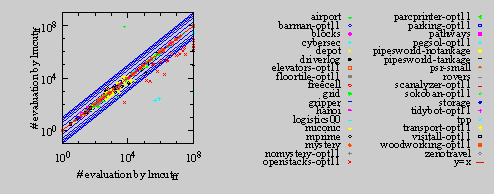
\includegraphics{tables/aaai16-30min/aaai16prelim3/evaluated-lmcut_ff-lmcut_lf.pdf}
 \caption{Comparisons of \# of Evaluations between simple \lifo and
 \fifo second-level tie-breaking, with first-level $h$ tie-breaking. Each
 line shows $\times 2,4,6\ldots$ boundary.}  \label{f-h-eval}
\end{figure}

According to \reftbl{single-coverage} (left) with $h$ tie-breaking, \lifo
outperforms \fifo.
\refig{f-h-eval} also shows that the difference in the number of nodes
evaluated can sometimes be larger than a factor of 10, especially in
Openstacks and Cybersec.

\subsubsection{Is $h$-Based Tie-Breaking necessary?}

Next, we investigated whether $h$-based, first-level tie-breaking is necessary.
In \reftbl{single-coverage} (right), which shows the results when  first-level
tie-breaking based on $h$ is disabled, $[f, \lifo]$, which simply breaks ties among nodes with the same $f$-cost by expanding most recently generated nodes first (first suggested in \cite{korf1985depth}),
clearly dominates $[f, \fifo]$.

Interestingly, the performance of the $[f, \lifo]$ strategy
is comparable to $[f,h,\lifo]$ and $[f,h,\fifo]$, the two-level strategies that first break ties according to $h$.
This is somewhat surprising, considering the ubiquity of $h$-based tie-breaking in the search and planning communities.
% 
This can be understood as \lifo behaves very similar to $h$
tie-breaking.  \lifo greedily explores the plateau space and quickly
increases the $g$ value. At the same time $h$ decrease quickly because $f$
is fixed within the plateau.
% \citeauthor{burns2012implementing}
% (\citeyear{burns2012implementing}) writes ``the goal can be found more
% quickly in the final $f$ layer of search'' about $h$ tie-breaking.

% Note that \lifo no longer requires the gradient provided by $h$.

\subsubsection{Plateaus and Tie-Breaking}

In the comparison
% of the simple two-level tie-breaking strategies
above, we observed that large differences in performance between
two-level tie-breaking strategies tend to occur in problems where
there are many nodes with the same $f$ and $h$ values, creating
large plateau regions where the heuristic does not provide
useful guidance -- in effect, these plateau regions in the last
frontier ($f=f^*$) by definition requires blind search, i.e., 
relying solely on the tie-breaking criterion.
%%%, in order to
%% in the final plateau, there is no need to escape the
%% plateau. ``escape'' is a word for inadmissible search. A* is never
%% allowed to escape the plateau until all nodes are expanded.
% escape the plateau and
%%% find a goal node.
%, i.e., the problems where the
%heuristic function is not informative and the planner relies heavily on
%the tie-breaking criteria.

\refig{plateau} plots the size of the final search plateau on 1104 IPC
benchmark instances \emph{with $h$ tie-breaking}.
The $y$-axis
represents the number of nodes with $[f,h]=[f^*,0]$, and the $x$-axis represents the total
number of nodes with $f\leq f^*$.
Clearly, in some domains such as Openstacks and Cybersec, the planner can spend most of the runtime
searching the final plateau.
It also
means that these domains have very large variance in the runtime caused
by the difference in second-level tie-breakings. 

%% Removed
% \refig{fig:plateau-noh} in the introduction is the same figure without $h$ tie-breaking.
% As expected, when the
% $h$-based tie-breaking is disabled in \refig{fig:plateau-noh}, much
% larger effort could be spent on the final plateau.

%  The size of the bucket does not change
% between $[f,h,\fifo]$, $[f,h,\lifo]$ and $[f,h,\ro]$.


\begin{figure}[tb]
 \centering \relsize{-3}
  % 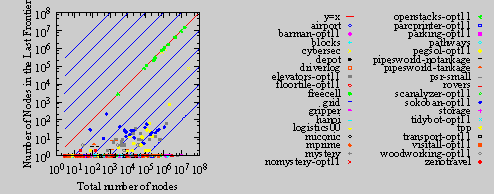
\includegraphics{tables/aaai16-frontier/aaai16prelim3/lmcut_frontier-front.pdf}
  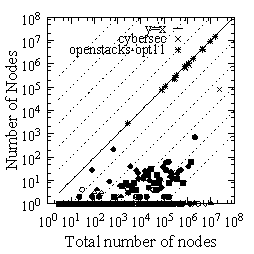
\includegraphics{tables/aaai16-frontier/aaai16prelim3/lmcut_frontier-front-mono.pdf}
  \caption{Comparing the size of the $[f,h]$ search plateau to the total
  evaluation below $f\leq f^*$. Data were obtained by the result of
  \lmcut on the standard benchmark instances. We do not show all labels
  for point types. Both axes are logarithmic. Dotted lines represent
  $\times 10^n$ boundaries.  Openstacks clearly has the large plateaus.}
  \label{plateau}
\end{figure}

\subsection{Domains with Zero-cost Actions}

%% best to put openstacks here, considering the connection to the
%% previous section
Openstacks domain is a cost
minimization domain first introduced in IPC-2006, where the objective is to 
minimize the number of stacks used.
There are many zero-cost actions (i.e., actions that don't increase the number of stacks), and
they prevent the standard heuristics from producing
informative guidance.
For example, \lmcut \cite{Helmert2009} fails to find a good cost
partitioning with non-zero values, 
% A detailed discussion of Openstacks domain and poor performance of landmarks is in \cite{richter10lama}, p.167-169.
and most edges in the abstraction
space of M\&S \cite{helmert2007flexible} have zero costs.

% XXX I'm commenting out the paragraphs below because:
% (1) A review of heuristic functions for domain-independent learning is not really
% necessary for this AAAI submission. 
% (2) It's better if this paper is not so strongly associated with the ICAPS community only -- this work applies in general to search with A*, and is not strongly tied to almost-perfect heuristics, lmcut, m&s, etc.

Such domains are
not common in the current set of benchmarks.
% 
Historically, the study of the shortest path finding algorithms has
started on the unit cost domains as the simplest case, where every
search edge has a cost 1,
% . Experimental study of \astar was somewhat biased to
% the unit-cost domains
such as 24-puzzle, Rubik's Cube etc.
% There are also several problems with non-unit costs, sometimes
% artificially but also sometimes naturally, such as in multiple
% sequence alignment (MSA).
% 
In the plannning community,
%  actions with non-unit costs were first introduced in 
% IPC-2002. The actions in these domains
actions tend to have the nonzero positive costs
because most domains target the runtime minimization.
% For example, Elevator and Miconic in the benchmark domains minimize the
% runtime of moving the passengers up and down.
% Actions in which the
% elevator travels the long distance take longer runtime.  
% When concerned
 % only with the runtime, it is reasonable to assign nonzero positive costs to
 % every actions
For runtime minimization,
nonzero positive costs are reasonable because
every actions are supposed to consume a fraction of time.
However, such formulation is not suitable for general optimization
problems.  For example, when you try to minimize the energy consumption
by the elevators in Elevators domain, many actions would have zero-cost
--- it does not consume electricity for either boarding or leaving the
passenger, or moving the elevator down.
% 
From the practical point of
view, cost minimization domains would have wider interest compared to
the simple runtime minimization.
Also, as shown previously, such domains pose a
difficulty to the current heuristic planners due to their large plateaus.

Therefore, in this paper, we modified various domains
into cost minimization domains with many zero-cost actions.
For example, elevators-up is a variation of
Elevators domain where the target is to minimize
the energy consumption caused by ``up'' action, which moves the elevator
up, and all other actions have zero-cost.  Modification was done in a
practically reasonable manner in a sense of cost minimization. Most
transportation-type domains are modified so that they use less
fuel (Logistics-fuel etc.). Assembly-type domains are modified so that it minimizes the
resource usage (Floortile-ink minimizes ink usage, or Woodworking-cut
minimizes wood usage, etc). For nontrivial domains, we selected one action
arbitrarily, and made other actions to have zero cost. We did not
include domains with single action schema and domains already with many
zero-cost actions.
We call this set of 29 domains as \emph{zerocost domains} hereafter.

% \todo[We also modify a same domain
% in the different minimization criteria, in order to avoid the bias on a
% particular domain formulation.]{It's not tested yet}

% This lack of general support for cost-minimization problems
% in the current competition domains can be fixed by
% % The same thing applies to the transportation-type and assembly-type
% % domains like Logistics and Woodworking, respectively. They are runtime
% % minimization domains in which driving and manual labor, or cutting and
% % painting, are equally measured by the single runtime metric.
% modifying some actions to have zero-cost.
% For example, Logistics and Woodworking, in which driving and manual labor, or cutting and
% painting, are equally measured by the single runtime metric,
% can be converted into
% cost-minimization domains in which the target is the fuel consumption
% (Logistics) or wood usage (Woodworking). 


% Currently, most benchmark domains except Openstacks and Cybersec do not
% have the large plateau thanks to the powerful heuristic estimates (which
% is verified in the later section). However, limiting our effective
% experiments only to 2 domains would bias our observation. To avoid this
% issue, we created several domains where the \sota heuristic functions
% fail to provide a menaingful guidance.

% One important characteristics shared by Openstacks and Cybersec is that they both
% have large number of zero-cost actions.
 % In such situations, both LMcut
% and M\&S fail to find a meaningful heuristic estimate because LMcut fails to
% find a good cost partitioning with non-zero values, and most edges in the abstraction space of
% M\&S have zero costs.

% We therefore modified various domains to have many zero-cost actions.
% For example, miconic-up is a domain which minimizes the energy
% consumption caused by ``up'' action, which moves the elevator up, and
% all other actions have zero-cost. Another example is driverlog-fuel, where only
% the ``drive'' action has cost 1 and all other actions are zero-cost.
% This in fact reflects the practical application compared to the original
% unit-cost domains where driving and manual labor is equally accounted.
% Oddly, although some planners have options which treats actions as if
% they are unit-costs, and describe such options as ``inadmissible'',
% solving domains which are unit-cost by origin is not called
% ``inadmissible''. Above modification addresses this problem.

We plotted the size of the final plateau of the zerocost domain instances just like in
\refig{plateau}. The trend of large plateaus becomes universal among
instances. Thus, in these cost-minimization problems, the search strategy within
plateau becomes much more important than in the
runtime-minimization problems.

\begin{figure}[tb]
 \centering \relsize{-3}
  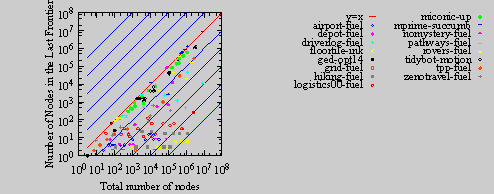
\includegraphics{tables/aaai16-frontier/zerocost/lmcut_frontier-front.pdf}
  \caption{Same plot as \refig{plateau}, but from the zerocost
  domains. Even with $h$ tie-breaking, zerocost domains force the planner
  to search much larger plateau.}
 \label{plateau-zerocost}
\end{figure}



\subsection{Depth-based Tie-Breaking}

In order to solve zerocost problems, the planner needs to run an
efficient knowledge-free search within the large final plateau.
One useful notion which can be used to both understand and control the
search in this situation is the \emph{depth} of a node, which represents
the number of steps from the entrance of the plateau.  Given a node $n$,
if its current parent $\parent{n}$ is from the other plateau, i.e.,
$\parent{n}$ has a different $f$-value, or different $h$-value when the
first tie-breaking is present, then $\depth{n} = 0$. Nodes with
$\depth{n} = 0$ are called the \emph{entrance} of the plateau.  If $n$
and $\parent{n}$ are in the same plateau and share the same $f$ and $h$,
$\depth{n}$ is defined as $\depth{\parent{n}} + 1$.  Based on this
simple notion of depth, we propose three \emph{depth-based
tie-breaking}, where the nodes are inserted to buckets associated with
depths, and upon expansion, the buckets are chosen in different manners.
FirstDepth(\fd), RandomDepth(\rd) and LastDepth(\ld) respectively break
ties by choosing a node from the bucket with the smallest depth, a
random depth, or the largest depth.

\todo{remove this part if complete plot in \refig{depth-histogram} did
not succeed}
The effectiveness of this second-level depth-based strategy depends on the
structure of the problem instance.  In the knowledge-free search within
the plateau, all nodes have the same $f$ and $h$ values
% yes, for simplicity, I'm assuming 3-level tiebreaks, ignoring no-h for the time being..
and it is impossible to guess whether the goal is concentrated near, far
away or in a particular step from the entrance.  In the first case, the
search should be focused around the entrance favoring the smaller depths
(FirstDepth), and the behavior in the plateau should be much like breadth-first. In the
second case, the planner should greedily explore the various area of the
plateau by preferring largest depth (LastDepth), much like in
depth-first. In the final case where the goal nodes are concentrated in
a particular depth, FirstDepth would take too much time to reach that
depth, and LastDepth would greedily go past and ignore the depth.
This is a case
where RandomDepth is the safest practice: 
Choosing the random depth will balance the exploration and exploitation
and maintains the possibility to expand the nodes in intermediate depths.

\subsubsection{Third-Level Tie-Breaking}

Since there can be multiple nodes with the same $f$, $h$ and depth,
a further tie-breaking criterion is necessary to select among nodes in the same depth bucket.
There are 3 possibilities in implementing this third-level tie-breaking:
\fifo, \lifo and Random Order (\ro), which
randomly selects an element from the depth bucket selected by the depth-based tie-breaking.

Among \fifo, \lifo and \ro, the natural policy is Random Order.
This is because the effectiveness of the third-level tie-breaking behavior
is affected by the accidental bias in action ordering in the PDDL domain
definition \cite{vallati2015effective}.
Finding the best action ordering is not the scope of this paper.
Thus, focusing on \ro and assess its expected/average
performance is the most reasonable practice to understand the behavior of second-level,
depth-based tie-breaking.

% Among \fifo, \lifo and \ro, the natural policy is Random Order.
% This is because the effectiveness of the third-level tie-breaking behavior
% is affected by the accidental bias in action ordering in the PDDL domain
% definition.  Recent work \cite{vallati2015effective} showed that the
% planner performance is greatly affected by changing and tuning the action ordering
% (and also variable ordering, but it is irrelevant to the tie-breaking behavior). 
% However, finding the best third-level tie-breaking is not the scope of this paper.
% Thus, focusing on \ro and assess its expected/average
% performance is the most reasonable practice to understand the behavior of second-level,
% depth-based tie-breaking.


\subsubsection{Evaluating Depth-based Tie-Breaking}

We evaluated five 3-level tie-breaking strategies and three 2-level
tie-breaking strategies in all.
%REDUNDANT? , i.e., $[f,h,depthStrategy,LFR]$, where the first-level tie-breaking is according to $h$ (break ties in favor of small $h$), the second-level strategy is based on depth and $depthStrategy \in \{\fd, \ld, \rd\}$, and the third level tie-breaking strategy $LFR \in \{\lifo, \fifo, \ro\}$.
% 
In addition to the 35 IPC benchmark domains with 1104 problems used in
the previous set of experiments, we used 29 zerocost domains with 640
problems.  \reftbl{depth} shows the coverage results. For randomized strategies, we
showed the mean and the standard deviation of the coverages obtained by
10 individual runs.

First, we compared $[f,h,\ld,\lifo]$ and $[f,h,\fd,\fifo]$
with $[f,h,\lifo]$ and $[f,h,\fifo]$, respectively, in order to see
the extra cost of managing the depth-based buckets.
The node evaluation order of $[f,h,\fd,\fifo]$ and $[f,h,\ld,\lifo]$
are exactly the same as $[f,h,\fifo]$ and $[f,h,\lifo]$.
This is because:
(1) $[f,h,\lifo]$ expands the most recently evaluated/inserted
states, and (2) the depth increases monotonically within the same $[f,h]$,
thus (3) $[f,h,\lifo]$ always expands the largest depth. (Similar logic
applies to $[f,h,\fifo]$.)
% 
% yet these results are useful in assessing the extra cost of managing the
% depth-based buckets.
As expected, the performances of $[f,h,\ld,\lifo]$ and
$[f,h,\fd,\fifo]$ are slightly worse than $[f,h,\lifo]$ and
$[f,h,\fifo]$, respectively, due to the cost of managing the depth-based buckets.

Next, we compared the performance of
$[f,h,\fd,\ro]$, $[f,h,\ld,\ro]$, $[f,h,\rd,\ro]$: Each using
$h$ as the first-level tie-breaking criterion, one of \fd, \ld, \rd as
the depth-based 2nd-level tie-breaking criterion, and finally,
\ro as the 3rd-level criterion.
Since these configurations involves randomness, we run 10
experiments with different random seeds for each configuration and
tested the significance of the difference of the mean coverage with Wilcoxon test,
a non-parametric significance testing method applicable to
the populations in which normal distribution cannot be assumed.

\reftbl{depth} shows the mean and standard deviation of the coverages,
along with 3 rightmost columns showing the $p$ values of the
test. The results depend on the domains, but in many situations we
observed a significant difference among 3 second-level tie-breaking, and
RandomDepth dominated the others. Although in most domains LastDepth and
RandomDepth behave similar, the performance of RandomDepth in some
domains are noticeable (e.g., Cybersec, Woodworking-cut). Also, the
standard deviation of the coverage results of RandomDepth tends to be smaller
than that of LastDepth, indicating the robustness of RandomDepth wrto seeds.
FirstDepth is dominated by the others, except in scanalyzer-analyse
and sokoban-pushgoal.

\todo{move this to the final section after revieweing the action ordering}
% removed \fifo
Finally, we answer two following concerns regarding \lifo final-level
tie-breaking criteria which appear in $[f,h,\lifo]$ and
$[f,h,\ld,\lifo]$. The re-evaluation in the earlier sections contains
two open questions: (1) Do the action orderings affect the performance of \lifo? 
(2) Doesn't \lifo benefit from its efficient low-level memory access pattern (high
probability of hitting the cache), not by the search efficiency?
They are both rejected because the
coverage of $[f,h,\ld,\lifo]=[f,h,\lifo]$ is not significantly
different from $[f,h,\ld,\ro]$, i.e.,
$859,857 \in [863.5-8.9,863.5+8.9]$,
despite the difference in the third-level tie-breaking (\lifo vs \ro).
% 
It means that the
performance of $[f,h,\lifo]$($=[f,h,\ld,\lifo]$) was not caused by the final-level
\lifo, but instead by the implicit second-level tie-breaking LastDepth.
%% remove
% Besides, this problem is not important now that RandomDepth
% is outperforming LastDepth-based tie-breaking strategy.
% 
With the similar logic, we can claim that the bad performance of
$[f,h,\fd,\fifo]$ and $[f,h,\fifo]$ can be attributed to its the
inherent second-level FirstDepth, and not to the third-level \fifo.
%% Unfortunately, 829,828 is not \in 816.7 +- 2.2.
%% this can be changed if we rerun _random with O(1) random deletion.

% Another issue in this result is the lack of analysis on
% abstraction-based heuristics. We also added the results in the figures
% in the supplemental materials. Above trends are mostly consistent when
% M\&S and blind heuristics are used, regardless of first-level
% tie-breaking by $h$-value. However, we note that many instances quickly
% exhausted the 2GB memory limit with those heuristics, and is less
% informative compared to the result by LMcut.

\begin{table}[tb]
 \centering
 \relsize{-3}
 \begin{tabular}{|c|c|c||c|c||c|c|c||c|c|c|}
\hline                              
 Domain & \rotatebox[origin=l]{90}{lmcut,ff}   & \rotatebox[origin=l]{90}{lmcut,lf}   & \rotatebox[origin=l]{90}{lmcut,fd,fifo}   & \rotatebox[origin=l]{90}{lmcut,ld,lifo}   & \rotatebox[origin=l]{90}{lmcut,fd,randomx}   & \rotatebox[origin=l]{90}{lmcut,ld,randomx}   & \rotatebox[origin=l]{90}{lmcut,rd,randomx}   & \rotatebox[origin=l]{90}{lmcut,fd,randomx}\rotatebox[origin=l]{90}{lmcut,ld,randomx}   & \rotatebox[origin=l]{90}{lmcut,fd,randomx}\rotatebox[origin=l]{90}{lmcut,rd,randomx}   & \rotatebox[origin=l]{90}{lmcut,ld,randomx}\rotatebox[origin=l]{90}{lmcut,rd,randomx}    \\
\hline                              
 sum(1104) &  558 &  565 &  557 &  565 &  554.6\spm{}0.8 &  568.3\spm{}1.8 &  570.6\spm{}1.5 &  0.0 &  0.0 &  .01  \\
\hline                              
 {\relsize{-1}cybersec(19)} &  2 &  3 &  2 &  3 &  2.0\spm{}0.0 &  7.3\spm{}1.5 &  9.6\spm{}1.1 &  0.0 &  0.0 &  .01  \\
 {\relsize{-1}openstacks-opt11(20)} &  11 &  18 &  11 &  18 &  10.0\spm{}0.0 &  18.0\spm{}0.0 &  18.0\spm{}0.0 &  0.0 &  0.0 &  1.0 \\\hline
 sum(380) &  163 &  164 &  163 &  163 &  157.4\spm{}1.2 &  167.9\spm{}4.8 &  172.8\spm{}1.7 &  0.0 &  0.0 &  .01  \\
\hline                              
 {\relsize{-1}driverlog-fuel(20)} &  8 &  8 &  8 &  7 &  8.0\spm{}0.0 &  7.2\spm{}0.7 &  8.0\spm{}0.0 &  .01 &  1.0 &  .01  \\
 {\relsize{-1}ged-opt14(20)} &  15 &  15 &  15 &  15 &  13.0\spm{}0.0 &  15.0\spm{}0.0 &  15.0\spm{}0.0 &  0.0 &  0.0 &  1.0  \\
 {\relsize{-1}miconic-up(30)} &  16 &  17 &  16 &  17 &  15.4\spm{}0.5 &  18.0\spm{}1.3 &  19.8\spm{}1.0 &  0.0 &  0.0 &  0.0  \\
 {\relsize{-1}mprime-succumb(35)} &  15 &  14 &  15 &  14 &  15.8\spm{}0.7 &  18.7\spm{}3.9 &  20.1\spm{}0.7 &  .18 &  0.0 &  .23  \\
 {\relsize{-1}pathways-fuel(30)} &  5 &  5 &  5 &  5 &  4.0\spm{}0.0 &  4.2\spm{}0.4 &  4.4\spm{}0.5 &  .17 &  .03 &  .37  \\
 {\relsize{-1}tpp-fuel(30)} &  8 &  11 &  8 &  11 &  7.0\spm{}0.0 &  11.0\spm{}0.0 &  11.0\spm{}0.0 &  0.0 &  0.0 &  1.0 \\\hline
 sum(260) &  108 &  130 &  108 &  129 &  104.7\spm{}1.0 &  127.3\spm{}3.4 &  129.4\spm{}2.3 &  0.0 &  0.0 &  .07  \\
\hline                              
 {\relsize{-1}elevators-up(20)} &  7 &  13 &  7 &  13 &  5.3\spm{}0.5 &  8.8\spm{}0.9 &  9.4\spm{}1.1 &  0.0 &  0.0 &  .25  \\
 {\relsize{-1}freecell-move(20)} &  4 &  19 &  4 &  19 &  4.0\spm{}0.0 &  19.4\spm{}0.5 &  16.5\spm{}0.7 &  0.0 &  0.0 &  0.0  \\
 {\relsize{-1}mystery-feast(20)} &  7 &  5 &  7 &  5 &  7.2\spm{}0.4 &  6.2\spm{}0.7 &  7.2\spm{}0.4 &  0.0 &  1.0 &  0.0  \\
 {\relsize{-1}pipesnt-pushstart(20)} &  8 &  8 &  8 &  8 &  8.0\spm{}0.0 &  8.6\spm{}1.3 &  9.8\spm{}0.4 &  .41 &  0.0 &  .04  \\
 {\relsize{-1}pipesworld-pushend(20)} &  3 &  4 &  3 &  4 &  3.0\spm{}0.0 &  4.2\spm{}1.0 &  4.5\spm{}0.8 &  0.0 &  0.0 &  0.5  \\
 {\relsize{-1}psr-small-open(20)} &  19 &  19 &  19 &  19 &  18.0\spm{}0.0 &  19.0\spm{}0.0 &  19.0\spm{}0.0 &  0.0 &  0.0 &  1.0  \\
 {\relsize{-1}scanalyzer-analyze(20)} &  9 &  9 &  9 &  9 &  9.7\spm{}0.6 &  9.3\spm{}0.5 &  9.1\spm{}0.3 &  .17 &  .02 &  0.3  \\
 {\relsize{-1}sokoban-pushgoal(20)} &  18 &  18 &  18 &  17 &  18.0\spm{}0.0 &  17.0\spm{}0.0 &  17.9\spm{}0.3 &  0.0 &  .37 &  0.0  \\
 {\relsize{-1}storage-lift(20)} &  4 &  4 &  4 &  4 &  4.0\spm{}0.0 &  5.0\spm{}1.2 &  4.4\spm{}0.5 &  .01 &  .03 &  .26  \\
 {\relsize{-1}woodworking-cut(20)} &  5 &  7 &  5 &  7 &  4.5\spm{}0.5 &  6.7\spm{}0.5 &  8.6\spm{}0.9 &  0.0 &  0.0 &  0.0 \\\hline
 total(1744) &  829 &  859 &  828 &  857 &  816.7\spm{}2.2 &  863.5\spm{}8.9 &  872.8\spm{}2.9 &  0.0 &  0.0 &  .01 \\\hline
\end{tabular}

 \caption{Experiments comparing the coverages of 7 configurations.
 Each cell shows the coverage of the domain solved with 5 min, 2GB
 setting. Zerocost domains are named as
 [original name]-[name of nonzero action].
 For the space reason, we omitted those domains in which all coverages are
 the same (deterministic configuration),
 or did not pass the Wilcoxon significance test under $p=0.05$ (randomized configuration).
 Full results are in the supplemental material.
}  \label{depth}
\end{table}

\begin{table}[tb]
 \centering \relsize{-3}
 \begin{tabular}{|c||c|c||c|}
\hline         
 Domain & \rotatebox[origin=l]{90}{lmcut,rx}   & \rotatebox[origin=l]{90}{lmcut,rd,randomx}   & \rotatebox[origin=l]{90}{lmcut,rx}\rotatebox[origin=l]{90}{lmcut,rd,randomx}    \\
\hline         
 sum(1104) &  559.8\spm{}1.0 &  570.6\spm{}1.5 &  0.0  \\
\hline         
 {\relsize{-1}cybersec(19)} &  4.4\spm{}1.0 &  9.6\spm{}1.1 &  0.0  \\
 {\relsize{-1}openstacks-opt11(20)} &  11.6\spm{}0.5 &  18.0\spm{}0.0 &  0.0 \\\hline
 sum(380) &  166.1\spm{}1.1 &  172.8\spm{}1.7 &  0.0  \\
\hline         
 {\relsize{-1}driverlog-fuel(20)} &  8.0\spm{}0.0 &  8.0\spm{}0.0 &  1.0  \\
 {\relsize{-1}ged-opt14(20)} &  15.0\spm{}0.0 &  15.0\spm{}0.0 &  1.0  \\
 {\relsize{-1}miconic-up(30)} &  17.0\spm{}0.4 &  19.8\spm{}1.0 &  0.0  \\
 {\relsize{-1}mprime-succumb(35)} &  17.9\spm{}0.5 &  20.1\spm{}0.7 &  0.0  \\
 {\relsize{-1}pathways-fuel(30)} &  4.4\spm{}0.5 &  4.4\spm{}0.5 &  1.0  \\
 {\relsize{-1}tpp-fuel(30)} &  8.1\spm{}0.3 &  11.0\spm{}0.0 &  0.0 \\\hline
 sum(260) &  113.8\spm{}1.2 &  129.4\spm{}2.3 &  0.0  \\
\hline         
 {\relsize{-1}elevators-up(20)} &  7.3\spm{}0.5 &  9.4\spm{}1.1 &  0.0  \\
 {\relsize{-1}freecell-move(20)} &  5.0\spm{}0.4 &  16.5\spm{}0.7 &  0.0  \\
 {\relsize{-1}mystery-feast(20)} &  7.3\spm{}0.5 &  7.2\spm{}0.4 &  .65  \\
 {\relsize{-1}pipesnt-pushstart(20)} &  8.5\spm{}0.5 &  9.8\spm{}0.4 &  0.0  \\
 {\relsize{-1}pipesworld-pushend(20)} &  3.9\spm{}0.3 &  4.5\spm{}0.8 &  .05  \\
 {\relsize{-1}psr-small-open(20)} &  19.0\spm{}0.0 &  19.0\spm{}0.0 &  1.0  \\
 {\relsize{-1}scanalyzer-analyze(20)} &  9.1\spm{}0.3 &  9.1\spm{}0.3 &  1.0  \\
 {\relsize{-1}sokoban-pushgoal(20)} &  18.0\spm{}0.0 &  17.9\spm{}0.3 &  .37  \\
 {\relsize{-1}storage-lift(20)} &  4.6\spm{}0.5 &  4.4\spm{}0.5 &  .41  \\
 {\relsize{-1}woodworking-cut(20)} &  7.1\spm{}0.3 &  8.6\spm{}0.9 &  0.0 \\\hline
 total(1744) &  839.7\spm{}2.1 &  872.8\spm{}2.9 &  0.0 \\\hline
\end{tabular}

 \caption{Comparison of the mean and standard deviation of coverages by
 the RandomOrder last-level tiebreaking with and
 without second-level depth tie-breaking, $[f,h,\ro]$ and $[f,h,\rd,\ro]$. Each cell
 shows the average coverage of the domain obtained by 10 runs with 5
 min, 2GB setting.  For the space reason, we omitted those domains in
 which the results are not significantly different under Wilcoxon test
 with $p=0.05$. Full results are available in the supplemental material.
 }  \label{r-vs-rd-random}
\end{table}

\subsubsection{Do the Action Orderings Affect the Performance of Tie-Breaking?}

Finally, we show that the performance of our depth-based tie-breaking is
not affected by the bias introduced in the action orderings in the PDDL
domain definition.  We created 3 individual sets of domains in which the
original names of action schema are uglyfied into random strings. This is because
the Fast Downward code base has a preprocessing
step which sorts the action schemas according to the dictionary
order, and it affects the order of the applicable actions of each search node.
Each set of domains contains all of the benchmark and zerocost
domains.

We tested our most successful tie-breaking method $[f,h,\rd,\ro]$ on each
set of randomized domains, three times each with different random seeds,
resulting in 9 runs in total. Note that the robustness wrto random seed is
already proven in the last section.

The coverage results are shown in \reftbl{actionordering-robustness}.
We analysed these results using statistical methods.
We first applied Bartlett test to test if the sample groups wrto each
set of randomized domains share the same variance.
% There is no significant difference between the variances of the sample
% groups with confidence $p=0.00 < 0.05$.
Due to the small sample size, 
we could not verify the homogeneity of variances ($p=0.70$).

% (ql:quickload :rcl)
% (use-package :rcl)
% (r-init)
% (r "bartlett.test" '((571 573 571) (572 572 570) (573 575 571)))

% Since the variances are the same, we applied one-way ANOVA to test if
% the sample groups have the same mean values.
%%
Since the variances are not the same, we applied 
non-parametric Kruskal-Wallis test to see if
there is any difference in the mean values between the sample groups.
The null hypothesis is retained ($p=0.47$) and the significant
difference was not observed.

% (ql:quickload :rcl)
% (use-package :rcl)
% (r-init)
% (r "kruskal.test" '((571 573 571) (572 572 570) (573 575 571)))

\begin{table}[tb]
 \centering \relsize{-3}
 %\begin{tabular}{|c||c|c||c|c|c||c|c|c||c|c|c||c|c|c|}
\hline                                          
 Domain & \rotatebox[origin=l]{90}{lmcut,ld,randomx}   & \rotatebox[origin=l]{90}{lmcut,rd,randomx}   & \rotatebox[origin=l]{90}{lmcut,ld,randomx,2280}   & \rotatebox[origin=l]{90}{lmcut,ld,randomx,2432}   & \rotatebox[origin=l]{90}{lmcut,ld,randomx,15314}   & \rotatebox[origin=l]{90}{lmcut,rd,randomx,2280}   & \rotatebox[origin=l]{90}{lmcut,rd,randomx,2432}   & \rotatebox[origin=l]{90}{lmcut,rd,randomx,15314}   & \rotatebox[origin=l]{90}{lmcut,ld,randomx,2280}   & \rotatebox[origin=l]{90}{lmcut,ld,randomx,2432}   & \rotatebox[origin=l]{90}{lmcut,ld,randomx,15314}   & \rotatebox[origin=l]{90}{lmcut,rd,randomx,2280}   & \rotatebox[origin=l]{90}{lmcut,rd,randomx,2432}   & \rotatebox[origin=l]{90}{lmcut,rd,randomx,15314}    \\
\hline                                          
 sum(1104) &  568.0\spm{}1.4 &  571.7\spm{}0.9 &  567 &  567 &  570 &  571 &  573 &  571 &  53453876429 &  53453445617 &  53153939944 &  53054630959 &  52855052463 &  53055118088 \\\hline
 sum(380) &  172.7\spm{}2.1 &  169.7\spm{}0.5 &  173 &  175 &  170 &  170 &  169 &  170 &  20745209155 &  20554935065 &  21038450133 &  21044249397 &  21139379995 &  21045425987 \\\hline
 sum(260) &  130.0\spm{}2.8 &  127.0\spm{}0.8 &  126 &  132 &  132 &  128 &  126 &  127 &  13135650022 &  12538926357 &  12539913452 &  12953782527 &  13146086022 &  13041215376 \\\hline
 sum(1104) &  568.0\spm{}1.4 &  571.7\spm{}0.9 &  567 &  567 &  570 &  571 &  573 &  571 &  53154445513 &  53154525092 &  53353719312 &  52954806534 &  52954410880 &  53154246049 \\\hline
 sum(380) &  172.7\spm{}2.1 &  169.7\spm{}0.5 &  173 &  175 &  170 &  170 &  169 &  170 &  20745376136 &  20555172324 &  21038588895 &  20845700303 &  20744544273 &  20742668307 \\\hline
 sum(260) &  130.0\spm{}2.8 &  127.0\spm{}0.8 &  126 &  132 &  132 &  128 &  126 &  127 &  13325387377 &  12331490437 &  12830251681 &  12555898212 &  13138649739 &  12267203886 \\\hline
 sum(1104) &  568.0\spm{}1.4 &  571.7\spm{}0.9 &  567 &  567 &  570 &  571 &  573 &  571 &  53154844965 &  53154545412 &  53054498298 &  52854208990 &  52654902163 &  53054545808 \\\hline
 sum(380) &  172.7\spm{}2.1 &  169.7\spm{}0.5 &  173 &  175 &  170 &  170 &  169 &  170 &  20745213348 &  20554939144 &  21038454659 &  20941436904 &  20941330432 &  20857182304 \\\hline
 sum(260) &  130.0\spm{}2.8 &  127.0\spm{}0.8 &  126 &  132 &  132 &  128 &  126 &  127 &  13227678250 &  12531692255 &  12831380301 &  12952354353 &  12761488656 &  12948386130 \\\hline
\end{tabular}

 %\begin{tabular}{|c||c|c|c||c|c|c|}
\hline                  
 Domain & \rotatebox[origin=l]{90}{lmcut,rd,randomx,2280}   & \rotatebox[origin=l]{90}{lmcut,rd,randomx,2432}   & \rotatebox[origin=l]{90}{lmcut,rd,randomx,15314}   & \rotatebox[origin=l]{90}{lmcut,rd,randomx,2280}   & \rotatebox[origin=l]{90}{lmcut,rd,randomx,2432}   & \rotatebox[origin=l]{90}{lmcut,rd,randomx,15314}    \\
\hline                  
 sum(1104) &  571 &  573 &  571 &  53054630959 &  52855052463 &  53055118088 \\\hline
 sum(1104) &  571 &  573 &  571 &  52954806534 &  52954410880 &  53154246049 \\\hline
 sum(1104) &  571 &  573 &  571 &  52854208990 &  52654902163 &  53054545808 \\\hline
 sum(380) &  170 &  169 &  170 &  21044249397 &  21139379995 &  21045425987 \\\hline
 sum(380) &  170 &  169 &  170 &  20845700303 &  20744544273 &  20742668307 \\\hline
 sum(380) &  170 &  169 &  170 &  20941436904 &  20941330432 &  20857182304 \\\hline
 sum(260) &  128 &  126 &  127 &  12953782527 &  13146086022 &  13041215376 \\\hline
 sum(260) &  128 &  126 &  127 &  12555898212 &  13138649739 &  12267203886 \\\hline
 sum(260) &  128 &  126 &  127 &  12952354353 &  12761488656 &  12948386130 \\\hline
\end{tabular}

 \begin{tabular}{|c||c|c|c||c|c|c|}
\hline                  
 Domain & \rotatebox[origin=l]{90}{lmcut,rd,randomx,2280}   & \rotatebox[origin=l]{90}{lmcut,rd,randomx,2432}   & \rotatebox[origin=l]{90}{lmcut,rd,randomx,15314}   & \rotatebox[origin=l]{90}{lmcut,rd,randomx,2280}   & \rotatebox[origin=l]{90}{lmcut,rd,randomx,2432}   & \rotatebox[origin=l]{90}{lmcut,rd,randomx,15314}    \\
\hline                  
 sum(1104) &  571 &  573 &  571 &  53054630959 &  52855052463 &  53055118088 \\\hline
 sum(1104) &  571 &  573 &  571 &  52954806534 &  52954410880 &  53154246049 \\\hline
 sum(1104) &  571 &  573 &  571 &  52854208990 &  52654902163 &  53054545808 \\\hline
 sum(380) &  170 &  169 &  170 &  21044249397 &  21139379995 &  21045425987 \\\hline
 sum(380) &  170 &  169 &  170 &  20845700303 &  20744544273 &  20742668307 \\\hline
 sum(380) &  170 &  169 &  170 &  20941436904 &  20941330432 &  20857182304 \\\hline
 sum(260) &  128 &  126 &  127 &  12953782527 &  13146086022 &  13041215376 \\\hline
 sum(260) &  128 &  126 &  127 &  12555898212 &  13138649739 &  12267203886 \\\hline
 sum(260) &  128 &  126 &  127 &  12952354353 &  12761488656 &  12948386130 \\\hline
\end{tabular}

 \caption{Results showing the total coverages with
 three seeds on three uglified versions of the same set of domains. The effect
 of action ordering in the domain definition is so small that it does not
 affect the coverage. In contrast, $[f,h,\lifo]$ is greatly affected by
 the action ordering. TODO}
 \label{actionordering-robustness}
\end{table}

\subsubsection{How Depth-based Tie-breakings Perform without $h$ Tie-Breaking?}

In earlier sections, we showed that $[f,\lifo]$ tie-breaking is
sufficient for solving the benchmark instances, and $h$ tie-breaking may
not be necessary. We further strengthen our claim by showing the results
of $[f,\rd,\ro]$. In \reftbl{rd-without-h}, we see that $[f,\rd,\ro]$
dominates the other strategies, including those with $h$ tie-breaking.

\begin{table}[tb]
 \centering \relsize{-3}
 %\begin{tabular}{|c|c|c||c|}
\hline         
 Domain & \rotatebox[origin=l]{90}{lmcut,ff}   & \rotatebox[origin=l]{90}{lmcut,lf}   & \rotatebox[origin=l]{90}{lmcut,rd,randomx,noh}    \\
\hline         
 sum(1104) &  558 &  565 &  560.0\spm{}0.9  \\
\hline         
 {\relsize{-1}airport(50)} &  27 &  26 &  21.0\spm{}0.0  \\
 {\relsize{-1}barman-opt11(20)} &  0 &  0 &  0.0\spm{}0.0  \\
 {\relsize{-1}blocks(35)} &  28 &  28 &  27.0\spm{}0.0  \\
 {\relsize{-1}cybersec(19)} &  2 &  3 &  7.8\spm{}0.7  \\
 {\relsize{-1}depot(22)} &  6 &  6 &  6.0\spm{}0.0  \\
 {\relsize{-1}driverlog(20)} &  13 &  13 &  13.0\spm{}0.0  \\
 {\relsize{-1}elevators-opt11(20)} &  15 &  15 &  14.8\spm{}0.4  \\
 {\relsize{-1}floortile-opt11(20)} &  6 &  6 &  6.0\spm{}0.0  \\
 {\relsize{-1}freecell(80)} &  9 &  9 &  9.0\spm{}0.0  \\
 {\relsize{-1}grid(5)} &  1 &  1 &  1.0\spm{}0.0  \\
 {\relsize{-1}gripper(20)} &  6 &  6 &  6.0\spm{}0.0  \\
 {\relsize{-1}hanoi(30)} &  12 &  12 &  12.0\spm{}0.0  \\
 {\relsize{-1}logistics00(28)} &  20 &  20 &  20.0\spm{}0.0  \\
 {\relsize{-1}miconic(150)} &  140 &  140 &  135.6\spm{}0.5  \\
 {\relsize{-1}mprime(35)} &  21 &  21 &  21.0\spm{}0.0  \\
 {\relsize{-1}mystery(30)} &  15 &  16 &  15.8\spm{}0.4  \\
 {\relsize{-1}nomystery-opt11(20)} &  14 &  14 &  13.8\spm{}0.4  \\
 {\relsize{-1}openstacks-opt11(20)} &  11 &  18 &  18.0\spm{}0.0  \\
 {\relsize{-1}parcprinter-opt11(20)} &  13 &  13 &  13.0\spm{}0.0  \\
 {\relsize{-1}parking-opt11(20)} &  1 &  1 &  1.0\spm{}0.0  \\
 {\relsize{-1}pathways(30)} &  5 &  5 &  5.0\spm{}0.0  \\
 {\relsize{-1}pegsol-opt11(20)} &  17 &  17 &  17.0\spm{}0.0  \\
 {\relsize{-1}pipesworld-notankage(50)} &  15 &  14 &  14.2\spm{}0.4  \\
 {\relsize{-1}pipesworld-tankage(50)} &  8 &  8 &  8.0\spm{}0.0  \\
 {\relsize{-1}psr-small(50)} &  48 &  48 &  48.0\spm{}0.0  \\
 {\relsize{-1}rovers(40)} &  7 &  7 &  7.0\spm{}0.0  \\
 {\relsize{-1}scanalyzer-opt11(20)} &  10 &  10 &  9.0\spm{}0.0  \\
 {\relsize{-1}sokoban-opt11(20)} &  19 &  19 &  19.0\spm{}0.0  \\
 {\relsize{-1}storage(30)} &  14 &  14 &  14.4\spm{}0.5  \\
 {\relsize{-1}tidybot-opt11(20)} &  12 &  12 &  11.8\spm{}0.4  \\
 {\relsize{-1}tpp(30)} &  6 &  6 &  6.0\spm{}0.0  \\
 {\relsize{-1}transport-opt11(20)} &  6 &  6 &  6.0\spm{}0.0  \\
 {\relsize{-1}visitall-opt11(20)} &  10 &  10 &  10.0\spm{}0.0  \\
 {\relsize{-1}woodworking-opt11(20)} &  10 &  10 &  11.8\spm{}0.4  \\
 {\relsize{-1}zenotravel(20)} &  11 &  11 &  11.0\spm{}0.0 \\\hline
 sum(380) &  163 &  164 &  168.4\spm{}2.6  \\
\hline         
 {\relsize{-1}airport-fuel(20)} &  15 &  13 &  10.4\spm{}0.5  \\
 {\relsize{-1}depot-fuel(22)} &  6 &  6 &  6.0\spm{}0.0  \\
 {\relsize{-1}driverlog-fuel(20)} &  8 &  8 &  8.0\spm{}0.0  \\
 {\relsize{-1}floortile-ink(20)} &  8 &  8 &  8.0\spm{}0.0  \\
 {\relsize{-1}ged-opt14(20)} &  15 &  15 &  14.2\spm{}0.7  \\
 {\relsize{-1}grid-fuel(5)} &  1 &  1 &  1.0\spm{}0.0  \\
 {\relsize{-1}hiking-fuel(20)} &  9 &  9 &  9.0\spm{}0.0  \\
 {\relsize{-1}logistics00-fuel(28)} &  16 &  16 &  16.0\spm{}0.0  \\
 {\relsize{-1}miconic-up(30)} &  16 &  17 &  20.4\spm{}1.0  \\
 {\relsize{-1}mprime-succumb(35)} &  15 &  14 &  18.6\spm{}2.0  \\
 {\relsize{-1}nomystery-fuel(20)} &  10 &  10 &  9.4\spm{}0.5  \\
 {\relsize{-1}pathways-fuel(30)} &  5 &  5 &  4.8\spm{}0.4  \\
 {\relsize{-1}rovers-fuel(40)} &  8 &  8 &  9.0\spm{}0.0  \\
 {\relsize{-1}tidybot-motion(20)} &  16 &  16 &  15.6\spm{}0.5  \\
 {\relsize{-1}tpp-fuel(30)} &  8 &  11 &  11.0\spm{}0.0  \\
 {\relsize{-1}zenotravel-fuel(20)} &  7 &  7 &  7.0\spm{}0.0 \\\hline
 sum(260) &  108 &  130 &  126.0\spm{}2.5  \\
\hline         
 {\relsize{-1}blocks-stack(20)} &  17 &  17 &  16.0\spm{}0.0  \\
 {\relsize{-1}elevators-up(20)} &  7 &  13 &  8.2\spm{}0.7  \\
 {\relsize{-1}freecell-move(20)} &  4 &  19 &  16.6\spm{}0.8  \\
 {\relsize{-1}gripper-move(20)} &  7 &  7 &  7.0\spm{}0.0  \\
 {\relsize{-1}mystery-feast(20)} &  7 &  5 &  7.2\spm{}0.7  \\
 {\relsize{-1}parking-movecc(20)} &  0 &  0 &  0.0\spm{}0.0  \\
 {\relsize{-1}pipesnt-pushstart(20)} &  8 &  8 &  9.8\spm{}0.4  \\
 {\relsize{-1}pipesworld-pushend(20)} &  3 &  4 &  5.4\spm{}0.8  \\
 {\relsize{-1}psr-small-open(20)} &  19 &  19 &  19.0\spm{}0.0  \\
 {\relsize{-1}scanalyzer-analyze(20)} &  9 &  9 &  7.4\spm{}1.0  \\
 {\relsize{-1}sokoban-pushgoal(20)} &  18 &  18 &  17.0\spm{}0.0  \\
 {\relsize{-1}storage-lift(20)} &  4 &  4 &  4.6\spm{}0.5  \\
 {\relsize{-1}woodworking-cut(20)} &  5 &  7 &  7.8\spm{}0.7 \\\hline
 total(1744) &  829 &  859 &  854.4\spm{}4.0 \\\hline
\end{tabular}

 \begin{tabular}{|c|c|c||c|}
\hline         
 Domain & \rotatebox[origin=l]{90}{lmcut,ff}   & \rotatebox[origin=l]{90}{lmcut,lf}   & \rotatebox[origin=l]{90}{lmcut,rd,randomx,noh}    \\
\hline         
 sum(1104) &  558 &  565 &  560.0\spm{}0.9  \\
\hline         
 {\relsize{-1}airport(50)} &  27 &  26 &  21.0\spm{}0.0  \\
 {\relsize{-1}blocks(35)} &  28 &  28 &  27.0\spm{}0.0  \\
 {\relsize{-1}cybersec(19)} &  2 &  3 &  7.8\spm{}0.7  \\
 {\relsize{-1}elevators-opt11(20)} &  15 &  15 &  14.8\spm{}0.4  \\
 {\relsize{-1}miconic(150)} &  140 &  140 &  135.6\spm{}0.5  \\
 {\relsize{-1}mystery(30)} &  15 &  16 &  15.8\spm{}0.4  \\
 {\relsize{-1}nomystery-opt11(20)} &  14 &  14 &  13.8\spm{}0.4  \\
 {\relsize{-1}openstacks-opt11(20)} &  11 &  18 &  18.0\spm{}0.0  \\
 {\relsize{-1}pipesworld-notankage(50)} &  15 &  14 &  14.2\spm{}0.4  \\
 {\relsize{-1}scanalyzer-opt11(20)} &  10 &  10 &  9.0\spm{}0.0  \\
 {\relsize{-1}storage(30)} &  14 &  14 &  14.4\spm{}0.5  \\
 {\relsize{-1}tidybot-opt11(20)} &  12 &  12 &  11.8\spm{}0.4  \\
 {\relsize{-1}woodworking-opt11(20)} &  10 &  10 &  11.8\spm{}0.4 \\\hline
 sum(380) &  163 &  164 &  168.4\spm{}2.6  \\
\hline         
 {\relsize{-1}airport-fuel(20)} &  15 &  13 &  10.4\spm{}0.5  \\
 {\relsize{-1}ged-opt14(20)} &  15 &  15 &  14.2\spm{}0.7  \\
 {\relsize{-1}miconic-up(30)} &  16 &  17 &  20.4\spm{}1.0  \\
 {\relsize{-1}mprime-succumb(35)} &  15 &  14 &  18.6\spm{}2.0  \\
 {\relsize{-1}nomystery-fuel(20)} &  10 &  10 &  9.4\spm{}0.5  \\
 {\relsize{-1}pathways-fuel(30)} &  5 &  5 &  4.8\spm{}0.4  \\
 {\relsize{-1}rovers-fuel(40)} &  8 &  8 &  9.0\spm{}0.0  \\
 {\relsize{-1}tidybot-motion(20)} &  16 &  16 &  15.6\spm{}0.5  \\
 {\relsize{-1}tpp-fuel(30)} &  8 &  11 &  11.0\spm{}0.0 \\\hline
 sum(260) &  108 &  130 &  126.0\spm{}2.5  \\
\hline         
 {\relsize{-1}blocks-stack(20)} &  17 &  17 &  16.0\spm{}0.0  \\
 {\relsize{-1}elevators-up(20)} &  7 &  13 &  8.2\spm{}0.7  \\
 {\relsize{-1}freecell-move(20)} &  4 &  19 &  16.6\spm{}0.8  \\
 {\relsize{-1}mystery-feast(20)} &  7 &  5 &  7.2\spm{}0.7  \\
 {\relsize{-1}pipesnt-pushstart(20)} &  8 &  8 &  9.8\spm{}0.4  \\
 {\relsize{-1}pipesworld-pushend(20)} &  3 &  4 &  5.4\spm{}0.8  \\
 {\relsize{-1}scanalyzer-analyze(20)} &  9 &  9 &  7.4\spm{}1.0  \\
 {\relsize{-1}sokoban-pushgoal(20)} &  18 &  18 &  17.0\spm{}0.0  \\
 {\relsize{-1}storage-lift(20)} &  4 &  4 &  4.6\spm{}0.5  \\
 {\relsize{-1}woodworking-cut(20)} &  5 &  7 &  7.8\spm{}0.7 \\\hline
 total(1744) &  829 &  859 &  854.4\spm{}4.0 \\\hline
\end{tabular}

 \caption{Results comparing the (mean) coverages of $[f,h,\fifo]$,
 $[f,h,\lifo]$ and $[f,h,\rd,\ro]$.} \label{rd-without-h}
\end{table}

\subsubsection{Search Behavior within a Plateau}

To understand the behavior of RandomDepth, we plotted the histogram of
the depths of search nodes opened by RandomDepth in the final search
plateau until the solution is found.
\refig{depth-histogram} shows a result of $[f,h,\rd,\ro]$, modified to produce lots of outputs,
in Woodworking-Cut domain.
Large dots show the depth where the solution was found.
In this domain, the LastDepth could search arbitrarly longer path in the
plateau, which would ignore the nodes in the intermediate depth.
\todo{better to plot all solutions}

The figure also illustrates the behavior of RandomDepth: Although it
randomly selects from the \emph{current} set of nonempty buckets,
a new depth is found only when the largest-depth bucket is selected,
resulting in non-flat curves.
RandomDepth is balancing the search in the smaller depth and larger
depth, however finding the optimal balance is an interesting avenue of
future work.

\begin{figure}[tb]
 \centering \relsize{-3}
 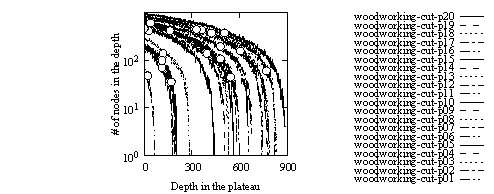
\includegraphics{tables/aaai16-log-rd/2zerocost/depth-histogram-lmcut_rdlog1-woodworking-cut.pdf}
 \caption{Histogram of the depths in the final search plateau.}
 \label{depth-histogram}
\end{figure}


\section{Related Work}
\label{sec-4}

Previous work on escaping search space plateaus has focused on
non-admissible search.  DBFS \cite{imai2011novel} is a technique which
adds stochastic backtracking to Greedy Best First Search to avoid
being misdirected by the heuristic function. Type based bucket
\cite{xie14type} classifies the plateau of GBFS according to the
$[g,h]$ pair and distributes the effort.  Marvin \cite{Coles07} learns plateau-escaping macros
from the Enhanced Hill Climbing phase of the FF planner
\cite{Hoffmann01} and later uses these macros to escape the plateau.
\citeauthor{Hoffmann05} gives a detailed analysis of the
structure of the search space in the benchmark domains which were
available in \citeyear{Hoffmann05} \cite{Hoffmann05,Hoffmann14}. 
The analysis was focused on the plateaus and dead ends which occur during the inadmissible search.
% 
However, to our knowledge, searching in plateaus has not been
previously investigated for cost-optimal planning with admissible
search.
The meaning of plateau in inadmissible and admissible search are
different in how to treat the non-final plateaus: Inadmissible search can
skip or escape a plateau whenever possible, while
admissible search cannot skip the remaining nodes in a plateau unless it
is the final plateau and it directly finds a solution.

In their work on combining multiple heuristics in a planner, \citeauthor{RogerH10}
(\citeyear{RogerH10}) considered a tie-breaking approach which works as follows:
When combining two heuristics, one of the
heuristics is used as the primary criterion for guiding the search,
and the second heuristic is used to break ties when the primary
heuristic values are the same for two states.
While this did not perform well in their work on satisficing planning, 
using a secondary heuristic as a tie-breaking criterion in our multi-level tie-breaking framework 
for cost-optimal search is an interesting direction for future work.

The PLUSONE\footnote{This term is used on the Fast Downward website.}
cost-type is a non-admissible search technique in the Fast Downward/LAMA planner
\cite{richter2010lama} which increases every action costs by 1.
By eliminating zero-cost actions, this has the effect similar to our
FirstDepth tie-breaking.
%Using PLUSONE, three successive
%applications of zero-cost operators have cost 3, and two
%applications have cost 2, and smaller cost is preferred, just as
%\astar always expands the node with smaller $f$-value.
This technique explicitly targeted zero-cost actions,
and resulted in a significantly better performance in IPC-6
satisficing track \cite[p.137, Sec. 3.3.2]{richter2010lama}.
\todo*{citation}
% There's a long discussion of Openstacks in \cite{richter2010lama}, p.167-169, but I can't find PLUSONE anywhere. Maybe it's called something else in the paper?  Maybe \richter2010lama is the wrong citation??

The major difference of our depth-based tie-breaking from PLUSONE
strategy is twofold.  First, depth-based tie-breaking is admissible,
because unlike PLUSONE, action costs are not modified.  Also, \emph{we
do not always favor smaller depth over larger depth}. LAMA treats the
increased cost as the part of sorting criteria and always prefers
smaller cost, much like in our FirstDepth strategy.  However, FirstDepth
strategy is the worst strategy in our experiments and the best
performing depth-based tie-breaking methods are LastDepth and RandomDepth
in our experiments, and they do not prefer the smaller depth.

% It's not clear what these techniques have in common, except that they are all orthogonal to heuristics,
% If that's the case, then there's no need to cite them in this paper -- there's no reason why these particular techniques
% are more relevant to this paper than hundreds of other techniques that are orthogonal to heuristics.
%% In admissible planning,
%% \emph{Symmetry Breaking}
%% \cite{Fox1998,pochter2011exploiting,domshlak2013symmetry} is the search
%% technique that tries to prune the states with symmetric
%% paths. \emph{Partial Order Reduction}
%% % , \emph{Strong Stubbern Sets} and \emph{Expansion Core} are
%% is also a technique which prunes the
%% intermediate states that reach to the same goal using the different
%% orders of same actions. \emph{Dominance Pruning} \cite{hall2013faster} is a
%% technique which prunes a state if it can be proven to be worse than the other nodes.
%% % 
%% These are usually not considered an attempt to improve the heuristic
%% estimates, however, in terms of \emph{Path-dependent globally admissible
%% heurisitics} \cite{karpas2012optimal}, a class of heuristics which is
%% admissible only on a particular optimal path, generalizes the above
%% techniques as assigining an infinite cost to some nodes on the other optimal paths.
%% % 
%% % From a slightly different category, Pathmax \cite{mero1984heuristic} and
%% % Bidirectional Pathmax \cite{felner2011inconsistent} are the techniques
%% % which converts an inconsistent heuristics into non-decreasing,
%% % consistent heuristics.
%% Thus, in a broad term, all of these methods are the
%% attempts to improve the heuristic estimates.
%% % Although in some particular
%% % case they may be able to return a perfect heuristics, they are still not
%% % always a perfect heuristics, implying that the plateau is unavoidable.
%% In contrast, our tie-breaking techniques aims specifically at the case
%% where the plateau is encountered and the planners are forced to run a
%% knowledge-free search.

$LA^*$ \cite{stern2010look} extends \astar by performing a
cost-bounded depth-first \emph{lookahead} from each node as it is generated.
Although this work was not done in the context of tie-breaking strategies, it is interesting to note that 
when the lookahead cost bound $k=0$ ($LA^*_0$ in their notation), only nodes with the same $f$-value as the current \astar frontier are expanded, which corresponds to a LastDepth strategy.

Vallati et al \shortcite{vallati2015effective} investigated the effect
of the ordering of objects (including operators, predicates, etc. ) in
PDDL domain models, and showed that orderings can have a significant
impact on planner performance in satisficing planning.
They conjectured that the reason for the performance variations caused
by object reordering is due to the impact of the tie-breaking,
% in \cite{vallati2015effective} p.7, col2, par#1
however it is not clear that the analysis can be
directly applicable to the admissible planning.
We avoided the effect of action orderings by using the randomized third
tie-breakings.
In contrast, we continued to use the variable ordering in the original domains
because the effect of variable ordering is irrelevant to the tie-breaking
criteria.

\section{Conclusion}

In this paper, we investigated the exisiting myth about the tie breaking
strategy of admissible search using \astar, and proposed a novel
depth-based tie-braking method which improves planner's performance in various
cost-minimization domains.
We showed that
our method is a heuristic-agnostic improvement which have a significant
impact on the search behavior in a large search plateau.
It also avoids the effect of action ordering in the domain definition,
providing a robust behavior.

 % when the distribution of optimal solutions is not uniform within the open list.
% We also showed that this nonuniform distribution still appears when we have almost-perfect % heuristics.

Our method differs from the pruning techniques because we do not prune
any states, nor from the other general improvements to the heuristic
accuracy because we just change the evaluation order within the same
$f$, yet it address the fundamental problems in the heuristic forward
search. 
% 
Future work includes a development of learning technique for
adaptively altering the search behavior in the plateau.



